\documentclass{Rpd}

\usepackage[table]{xcolor}
\usepackage{array}
\usepackage{wasysym}
\usepackage{hyperref}
\usepackage{multirow}
%\usepackage{csquotes}

\begin{document}

\def\Sectitle{Section Title}%%This line can be removed if there is no
						%%section title

\def\copyrightyear{2021}%

\title[short Title]{Measurement of the Regener-Pfotzer maximum using different types of ionizing radiation detectors and a new telemetry system TF-ATMON}
\author[\textit{et~al}]{Jakub Kákona\footnote{Corresponding author: kakonjak@fel.cvut.cz},$^{ a}$,  Martina Lužová \,$^{ b}$, Martin Kákona \,$^{ b}$, Marek Sommer \,$^{ b}$, Martin Povišer \,$^{ b}$, Ondřej Ploc \,$^{ b}$, Roman Dvořák \,$^{ c}$, Iva Ambrožová\,$^{ b}$}
\address{$^{ a}$Czech Technical University in Prague, Faculty of Electrical Engineering, Prague, Czech Republic, $^{ b}$Department of Radiation Dosimetry, Nuclear Physics Institute of the CAS, Na Truhlářce 39/64, 180 00, Prague 8, Czech Republic, $^{ c}$ ThunderFly s.r.o., U Jatek 19, Soběslav  392 01, Czech Republic}

\date{Received on April 2, 2003, revised on November 19, 2003, accepted on December 22, 2003}

\begin{abstract}
The exact location of the Regener-Pfotzer maximum depends on many parameters such as atmospheric conditions, geographical locations, solar activity, and also the type of detected particles. Stratospheric balloons are a useful tool for the investigation of cosmic radiation at high altitudes and the tests of new detectors of cosmic radiation. Due to necessary data processing of data measured by instruments, the balloon gondola needs to carry, together with radiation detectors,  additional supplementary sensors measuring humidity, temperature, location and orientation, altitude, atmospheric pressure, acceleration etc. This was the reason why a new universal system TF-ATMON was developed. The system is based on using already existing tools of the PX4 open-source project that makes it possible, apart from data recording and monitoring, to solve other related issues - the possibility to trace the balloon gondola after the flight. The application was demonstrated on stratospheric balloon flight FIK 6. This flight  was unique because three different types of radiation detectors were used at one flight. It enabled us to compare the altitude of the Regener-Pfotzer maximum measured with different types of sensors sensitive to a different type of secondary cosmic radiation generated in the atmosphere.

\end{abstract}

\maketitle


\section{Introduction}

Particles of primary cosmic radiation with sufficient energy interact in the upper part of the atmosphere and generate showers of secondary cosmic radiation. With increasing depth of the atmosphere the intensity of primary radiation decreases whereas the secondary component increases. At an altitude of about 20 km the intensity of secondary cosmic radiation reaches its maximum, called the Pfotzer-Regener maximum \cite{Regener}, \cite{Pfotzer}. The maximum varies with geomagnetic vertical cutoff rigidity and with solar cycle and it is generally located at 15-27 km above sea level \cite{Bazilevskaya}.
In the past, several experiments were done with the aim to measure vertical profile of ionization in the atmosphere at various locations in the word, mainly using radiosondes consisting of Geiger tubes \cite{Bazilevskaya}, \cite{ionization_profile},\cite{Vertical_profile_measurements}, \cite{cosmic_ray_intensity}, \cite{Radioactivity_atmosphere}, or to characterize instruments’ response used for space-based missions \cite{Lawrence} \cite{Mukherjee} \cite{Timepix}.
Stratospheric balloons are a useful tool for the investigation of cosmic radiation at high altitudes (around and above the Regener-Pfotzer maximum region) and for the tests of new detectors of cosmic radiation.
However, the radiation measuring instruments need to be supplemented by other sensors measuring temperature, pressure, humidity, altitude, acceleration, etc.  All these sensors should be continuously monitored during the launch and the flight of the balloon to verify their proper function and theirthe values have to be recorded for further processing of all obtained data.

The universal system TF-ATMON, based on the use of existing tools of the open-source project PX4 and supplemented with an telemetry transmitter, enables it to monitor and record data during the flight and to trace the balloon. Its application is demonstrated on stratospheric balloon flight FIK-6 Fig. \ref{FIK-6_setup} various radiation detectors - Geiger-Mueller tubes, Si-diode based detector SPACEDOS, and scintillation detectors AIRDOS-C with inorganic scintillation crystals - were used to measure the vertical profile of cosmic radiation in the atmosphere.

\section{Materials and methods}

Since 2015 we launched several stratospheric balloons, the overview of flights is summarized in Table \ref{Flight_reliability}.The construction of balloon gondolas was designed for specific radiation detectors during previous flights. Balloon avionics was therefore built around the chosen detectors.
This concept led to a situation when every new flight meant a significant amount of work despite the fact that many components were recycled every year and used for the next one. The reason was the need to adapt the avionics to the innovative version of detectors.

Due to a relatively high value of payload it was necessary to ensure the return of the gondola every flight. The main construction criteria were as follows:


\begin{itemize}
\item Reliable transmission of information about the geographical location of the gondola
\item Good resistance to impact
\item Ensuring the function in temperatures far below zero
\end{itemize}


Despite the generally successful nature of all fights and the fact that the gondolas were always found, different technologies were tried to eliminate the partial shortcomings which emerged during balloon flights. During the last experimental flights these also included the way the data was recorded.

For this reason, the originally used telemetry system was made significantly more robust and an IoT LoRa transmitter was added to the system, making it possible to transmit the data necessary for tracing the gondola to the TheThingsNetwork. This way, a high reliability of finding the gondola and recording the data was ensured. In case of active detectors, it was also necessary that the flight trajectory was recorded synchronously with the supplementary quantities.


An overall overview of the success of the used technologies is summarized in the table \ref{Flight_reliability}.


\begin{table*}[t]
\processtable{Table summarising success of used technologies, with colours representing a degree of reliability: \newline \colorbox{red}{Failure} \colorbox{yellow}{Partial failure} \colorbox{green}{Correct function}.\label{Flight_reliability}}
{\begin{tabular}{p{0.1\textwidth} >{\centering\arraybackslash}p{0.12\textwidth} >{\centering\arraybackslash}p{0.12\textwidth} >{\centering\arraybackslash}p{0.12\textwidth} >{\centering\arraybackslash}p{0.15\textwidth} >{\centering\arraybackslash}p{0.15\textwidth} >{\centering\arraybackslash}p{0.15\textwidth}}\toprule
Flight & FIK-1 & FIK-2 & FIK-3 & FIK-4 & FIK-5 & FIK-6 \\\midrule
Location (year) & CZ (2015) & CZ (2017) & CZ (2018) & SE (2019) & CZ (2019) & CZ (2020) \\
Payload & \cellcolor{green} Candy detector, Web camera & \cellcolor{yellow} Candy detector, Web camera & \cellcolor{green} AIRDOS,
360 deg camera & \cellcolor{green} AIRDOS-C CRY19, SPACEDOS, G-M, Socrat-R & \cellcolor{green} AIRDOS-C
CRY19,SPACEDOS, G-M, 360 deg camera & \cellcolor{green} AIRDOS-C NaI(Tl), SPACEDOS, G-M, Ionmeter, 360 deg camera \\
Landing site & \cellcolor{yellow} vineyard Austria & \cellcolor{green} rapeseed field & \cellcolor{red} Poland & \cellcolor{yellow} swamp (Finland) & \cellcolor{green} forest & \cellcolor{red} railway corridor\\
Power source & \cellcolor{green} Li-ion 18650 accu & \cellcolor{yellow} Li-ion 18650 and li-pol accu & \cellcolor{yellow} Lithium primary cells and li-pol accu & \cellcolor{green} Lithium primary cells & \cellcolor{yellow} Lithium primary cells & \cellcolor{green} Li-ion 18650
accu \\
Telemetry system & \cellcolor{red} GSM & \cellcolor{yellow} GSM, 868 MHz Proprietary Modem & \cellcolor{yellow} SigFox,
868 MHz Proprietary Modem &  Outsourced & \cellcolor{green} LoRa, SigFox, SiK 433 MHz & \cellcolor{green} 2x LoRa, SiK 433 MHz \\
Rescue beacon & \cellcolor{green} 433 MHz CW & \cellcolor{green} 433 MHz CW & \cellcolor{green} 433 MHz CW &  Outsourced & \cellcolor{green} 433 MHz CW & \cellcolor{green} 433 MHz CW \\
Flight control computer & \cellcolor{yellow} Odroid-U2 & \cellcolor{yellow} Odroid-U2 & Not used & Not used/outsourced & \cellcolor{green} PX4, FMU v5 & \cellcolor{green} PX4, FMU v5 \\
\botrule
\end{tabular}}{}
\end{table*}


Apart from technologies used in gondolas a number of supplementary tools have undergone intensive development. For example, in order to find the balloon it was necessary to have an accurate real-time map of its position together with a prediction of the subsequent flight and the site of impact. In the case of the last two flights, FIK-5 and FIK-6, the habhub \cite{habhub_tracker} was used to track and predict the movement of stratospheric balloon.
As can be seen from the table \ref{Flight_reliability}, during the last flights the avionics was implemented using an UAV technology. It used the Pixhawk autopilot with PX4 firmware. Telemetry was implemented by a very reliable combination of LoRa modem and SiK modem. Power was provided by Li-ion 18650 batteries that also have a reliable flight history.



\subsection{Universal avionics}
Based on our experiences we have used the universal concept of avionics called TF-ATMON that makes it possible to connect different types of payloads and carry out various atmospheric measurements. Furthermore, it provides the detectors with basic services such as power supply, time, position and orientation information. Basic quantities that affect many types of measurements are also recorded, including temperature, pressure, humidity, magnetic field and acceleration. Flight computer provides a possibility to record data from experiments in a common log file. Therefore it is extremely useful for testing high-altitude cosmic radiation detectors and dosimeters. It also reduces the number of modifications in experiments (dosimeters) required for balloon flight.

The schematic diagram of the new avionics is summarized in the figure \ref{avionics_schematics}.


\begin{figure}%avionic
	\centerline{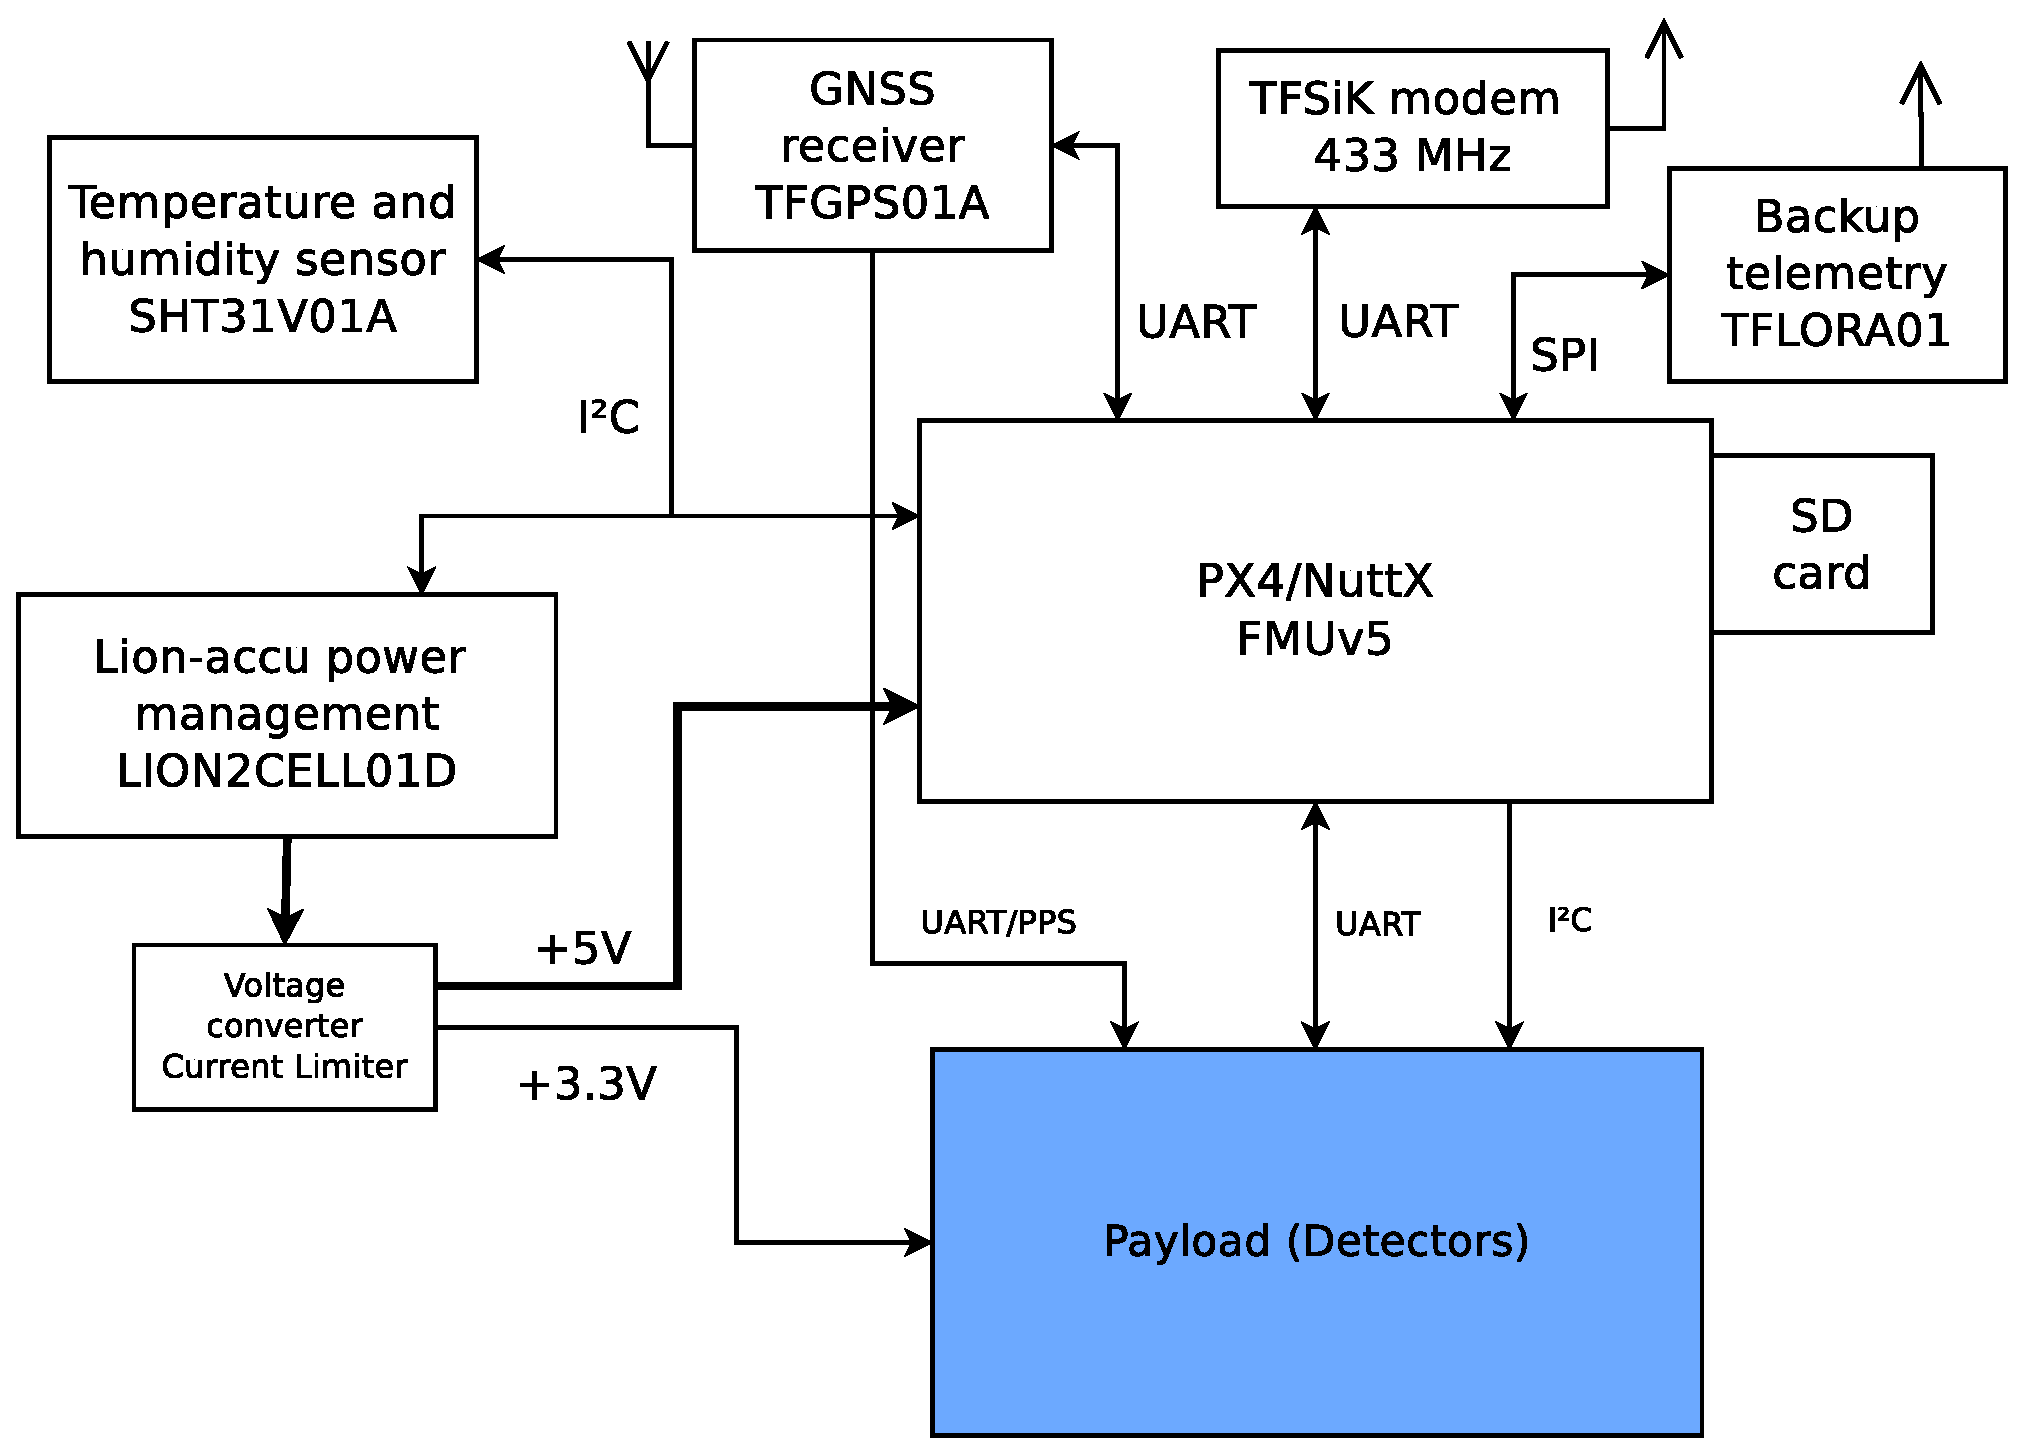
\includegraphics[width=60mm]{img/avionics_block_schematics.eps}}
	\caption{The schematic diagram of the new avionics \label{avionics_schematics}}
\end{figure}

Transition to the concept, where the balloon specific parts of avionics are completely separate from the system of detectors simplified the realization of next balloon flights. It reduced the complexity of connecting different types of detectors and at the same time it improved the integrity of supplementary data measurements. Overall, the new features can be summarized as follows:

\begin{itemize}
\item Easy implementation of different payloads
\item Redundant telemetry links
\item Gondola orientation and spatial position tracking and logging
\item Reliable IMU sensor processing and calibration
\item Possible use of relatively high-power consumption payloads
\item Pre-flight continuous charging as an option
\item Power monitoring and maximum uptime calculation relevant to actual temperature
\item Real-time pre-flight payload diagnostic
\end{itemize}

The documentation of used blocks can be found in the following sources TFGPS01 \cite{TFGPS01}, TFSIK01 \cite{TFSIK01}, TFHT01 \cite{TFHT01}, TFLORA01 \cite{TFLORA01}, \cite{LION2CELL01D}.


\subsection{Payload}

In the case of FIK-5 and FIK-6 flights that served as the test flights for our novel approach of using TF-ATMON technology the payload was not fully optimized for this use yet. All the detectors thus had their own SD cards for data recording and some even had their own power supply, therefore the payload weight was higher than theoretically required and some lift was wasted. This situation originated in conservative flight plan, which required successful log and function of payload even in failure of the new TF-ATMON system. Results from flight FIK-6 will be presented.

\subsubsection{Detectors}

The payload of FIK-6 flight contained TF-ATMON and three different types of ionizing radiation detectors: SPACEDOS with silicon PIN diode sensor (namely SPACEDOS02A), AIRDOS-C with scintillation crystal and silicon photomultiplier and a G-M tube. The total payload mass was 2 kg.

SPACEDOS is a lightweight dosimeter intended for space applications and measurements on board spacecraft. The detector has been described in \cite{SPACEDOS}. The detector is a silicon PIN diode with a volume $300$ µm $\times 10$ mm $\times 20$ mm $= 0.06$ cm$^3$. The energy range of this detector is from 0.2 MeV to 9 MeV.

AIRDOS-C is a scintillation detector with a small crystal. The detector has been described in \cite{AIRDOS-C}. This detector enhauses small cylindrical NaI(Tl) crystal with a volume $\diameter 10 mm \times 20 mm = 1.6$ cm$^3$ and SiPM (Silicon Photomultiplier) with a sensitive surface $6$ mm $\times 6$ mm. The energy range of this detector is from 0.2 MeV to 18 MeV.

The G-M tube STS-5 was used in the Geiger–Müller counter. The cylindrical volume of the tube is $\diameter 10$ mm$ \times 76$ mm $= 6$ cm$^3$. This detector is capable of registering the flux only. 

All detectors, together with other sensors and the TF-ATMON system were put inside a polystyrene box. 

\begin{figure}%avionic
	\centerline{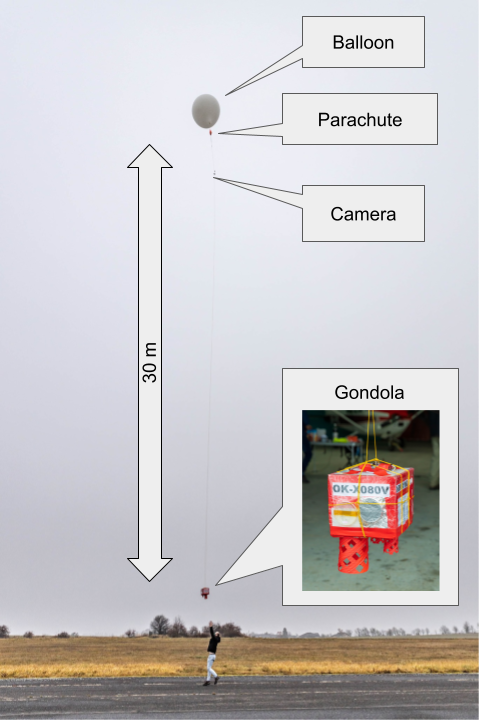
\includegraphics[width=50mm]{img/FIK-6_experiment_setup.png}}
	\caption{FIK-6 experiment setup using the Hwoyee Weather Balloon 1600. \label{FIK-6_setup}}
\end{figure}


\section{Results and discussion}

The flight FIK-6 took place on December 18th, 2020 and lasted 1 hour and 40 minutes. The balloon was launched from Pribram airport which is located around latitude 50$^{\circ}$ N. The balloon flight path continued in eastern direction for about 80km. 

The system TF-ATMON recorded temperature, air pressure, humidity and radiation characteristics as histograms of deposited energy of radiation events from all three radiation sensors in the gondola see Figure \ref{FIK-6_RAW_data}. The barometric altitude was calculated using the International Standard Atmosphere model 1976 \cite{standard_atmosphere}. 


\begin{figure}%avionic
	\centerline{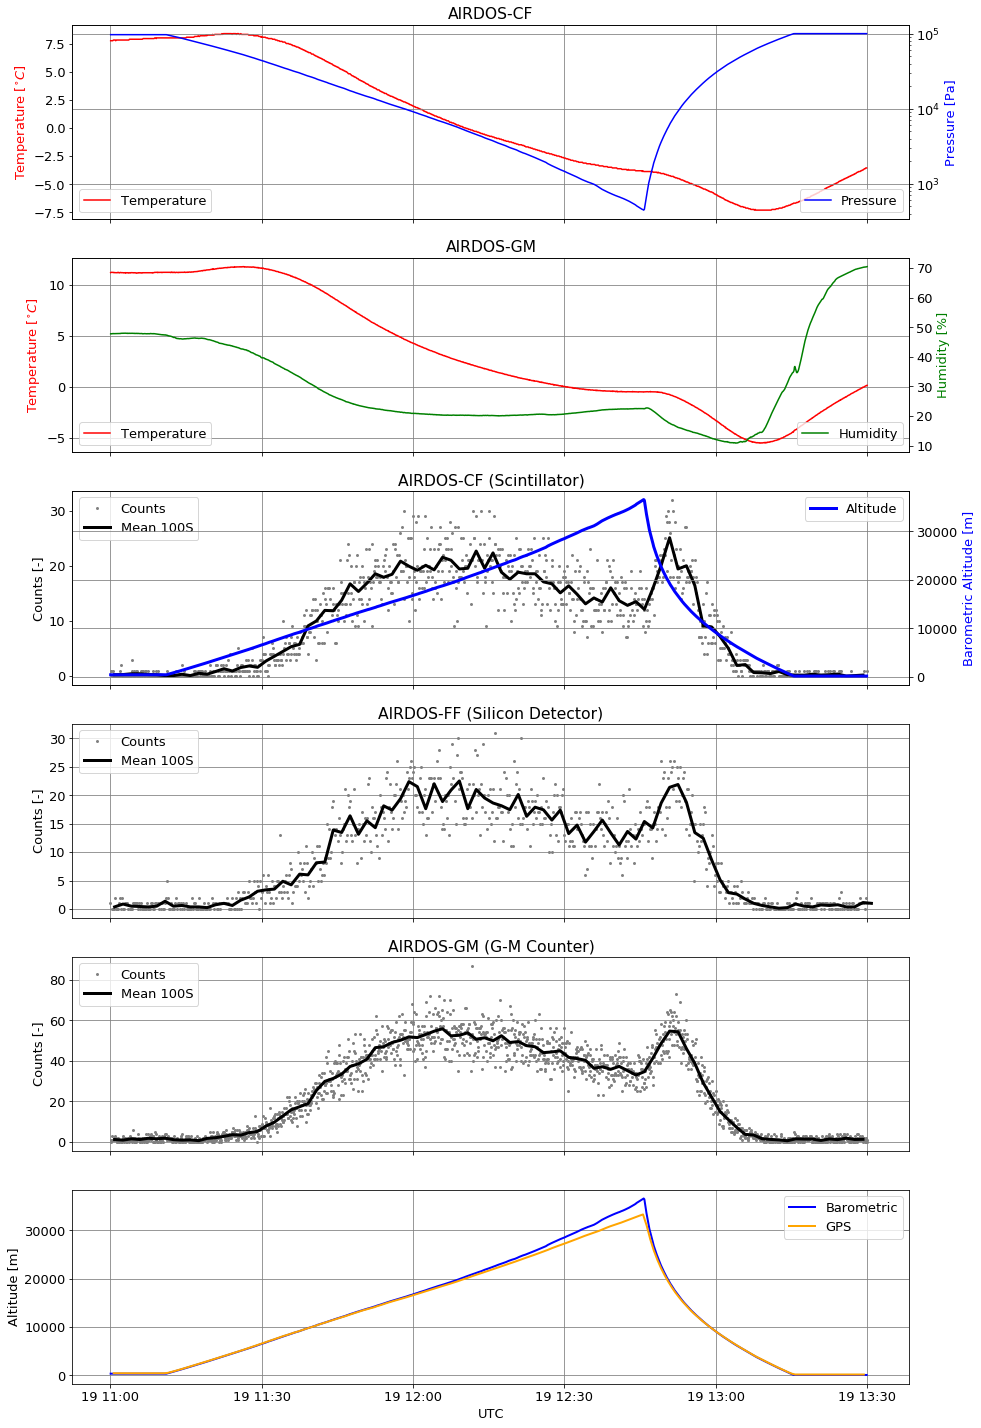
\includegraphics[width=60mm]{img/FIK-6_RAW_data.png}}
	\caption{Raw data measured during the whole flight. From top to bottom: temperature near scintillation crystal, air pressure inside the box of crystal, temperature inside the gondola, relative humidity inside the gondola, counts of radiation events per 10 seconds counted by scintillator, silicon detector, and  G-M counter, barometric altitude, and altitude from GNSS.\label{FIK-6_RAW_data}}
\end{figure}


\begin{figure}%avionic
	\centerline{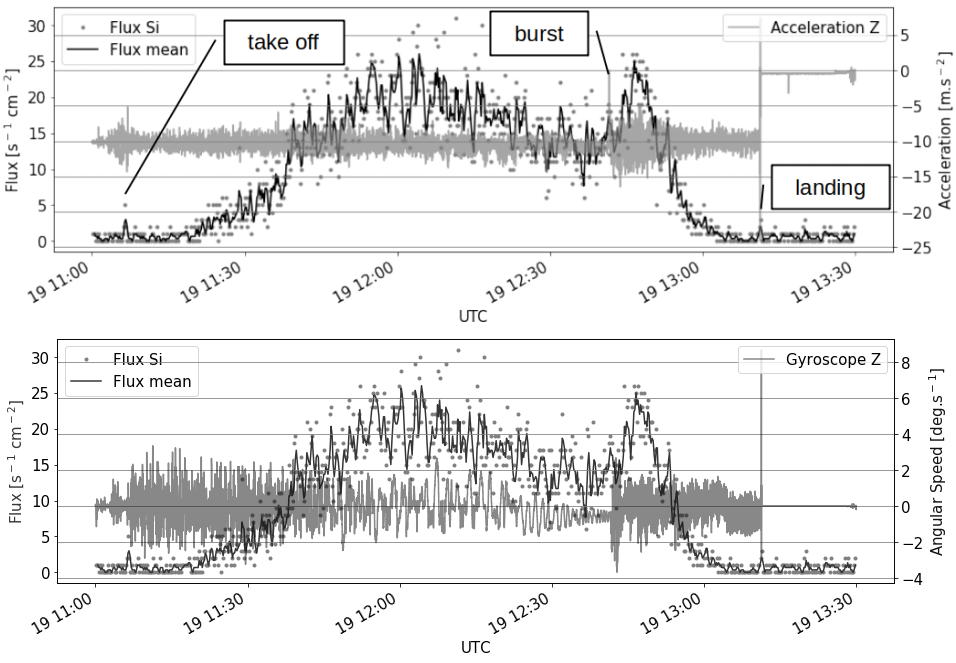
\includegraphics[width=60mm]{img/FIK-6_metadada.png}}
	\caption{Acceleration and Angular Speed in axis perpendicular to the ground combined with ionising radiation flux measured by the silicon PIN diode detector. \label{FIK-6_telemetry}}
\end{figure}

The picture \ref{FIK-6_telemetry} demonstrates the importance of telemetry data during measurements processing. The graphs show an increase in the response of the silicon ionizing radiation detector at the times of take off, burst and landing, when there was a rapid increase in mechanical stress. The effect is probably caused by the microphone effect of the silicon detector. Telemetry data provided by the TF-ATMON system must be therefore taken into account during data evaluation. The effect of these data on measured quantities will be a subject of further research. 


The graphs show that the maximum reached altitude was approximately 33km above sea level. During the flight the balloon passed the Regener-Pfotzer maximum twice. The rescue team followed the balloon along the whole flight trajectory. The precision of tracking allowed some participants of the rescue team to actually see the gondola touchdown visually. Therefore the gondola was successfully rescued within few minutes after touchdown Figure \ref{FIK-6_rescue_team}.

\begin{figure}%avionic
	\centerline{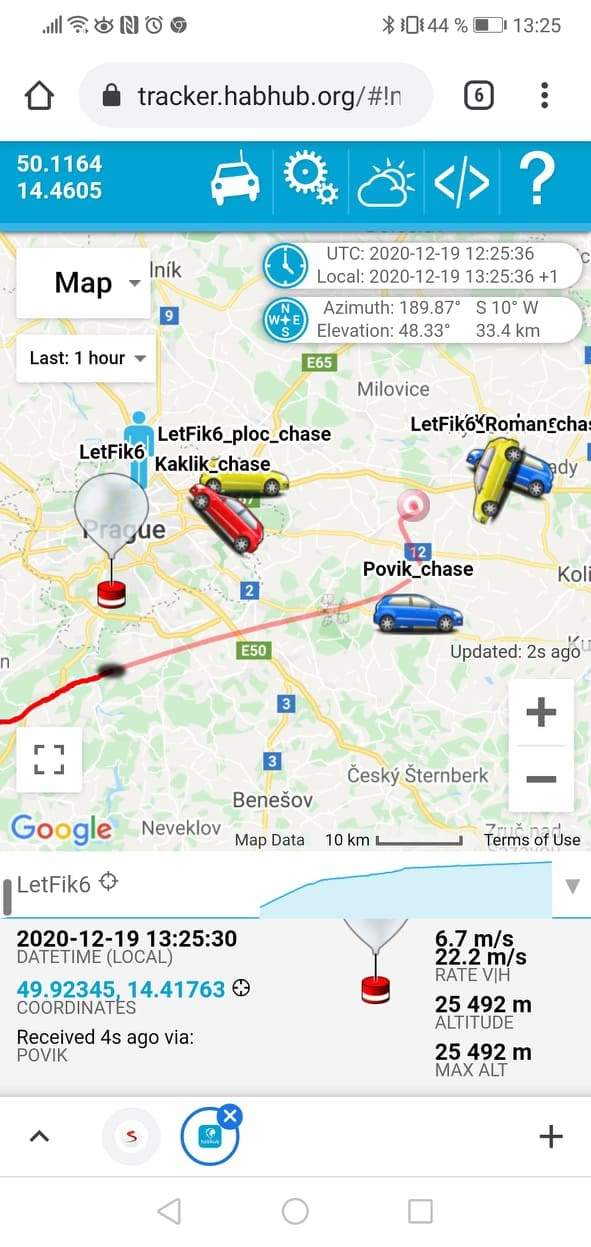
\includegraphics[width=40mm]{img/FIK-6_rescue_team.png}}
	\caption{Chasing cars with telemetry receivers at the landing site. \label{FIK-6_rescue_team}}
\end{figure}

By processing the data a graph of detected altitude Figure \ref{R-P_maximum} was obtained. It shows that the measured altitude of the Regener-Pfotzer maximum was for all detector types around 19km above sea level.

The Log-norm distribution fit was used to determine the R-P maximum. The fit was applied to measured data and normalized to the maximum number of particles for a given detector.

\begin{equation}A \frac 1 {x\sigma\sqrt{2\pi}}\ \exp\left( - \frac{\left(\ln x-\mu\right)^2}{2\sigma^2}\right)\end{equation}

The fit parameters $A$, $\mu$, $\sigma$ and the calculated R-P maximum positions are given in Figure \ref{R-P_maximum}. The range of barometric altitudes 7000 m to 29 000 m was chosen for the fit. The lower limit was chosen so that the course of the function was not affected by terrestrial radiation and radon progenies in the atmosphere. The upper limit was chosen based on a simulation because, according to the simulation, at higher altitudes the flux of ionizing radiation does not decrease evenly. 

Note that the absolute number of measured particles corresponds to the active volume, material and sensitivity of the used detector. The larger the volume the more particles. At the same time every detector measured a different position of R-P maximum. The lowest altitude was measured by the detector with the highest density (NaI(Tl), $\rho$ = 3.67 g/cm$^3$), followed by the silicon detector (Si, $\rho$ = 2.33 g/cm$^3$) and finally, the highest altitude of the maximum was measured by G-M tube (thin metallic tube filled with low pressure gas, the exact material composition of this tube is not known).

\begin{figure}
	\centerline{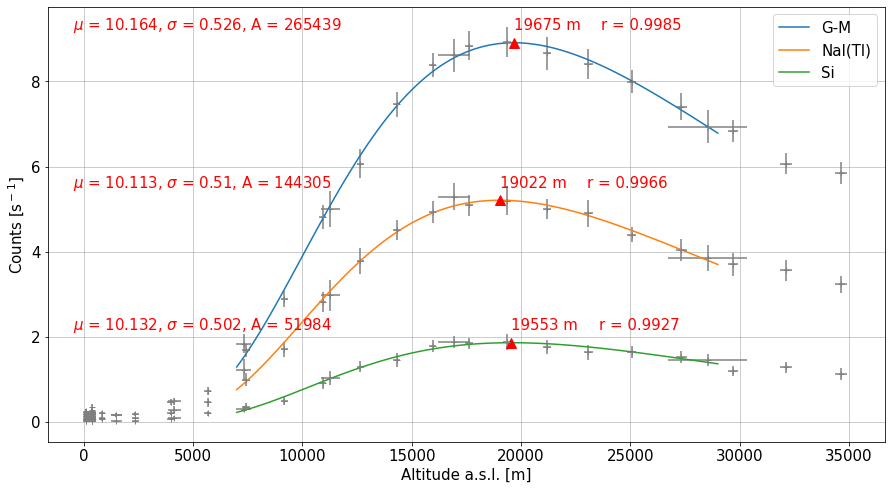
\includegraphics[width=70
	mm]{img/FIK-6_R-P_maximum.png}}
	\caption{Log-norm fit of ionising radiation measured data with calculated Regener-Pfotzer maxima for different detectors (G-M tube, NaI(Tl) scintillator and silicon PIN diode). Measured data are depicted with gray color as mean from 5 minutes of measurement with 2$\sigma$ standard errors. \label{R-P_maximum}}
\end{figure}

Altitudes of maxima of all three data sets were found using the log-normal fit (see Figure \ref{R-P_maximum}) described by mean value ($\mu_1$, $\mu_2$, $\mu_3$), variance ($\sigma_1$, $\sigma_2$, $\sigma_3$), and extent ($n_1$, $n_2$, $n_3$) where indexes 1, 2, and 3 refer to G-M counter, NaI(Tl) scintillator, and silicon PIN diode, respectively. We can see that altitudes of maxima differ. Statistical significance of this difference was evaluated using the two-selective testing of three hypotheses ($\mu_1 = \mu_2$, $\mu_1 = \mu_3$, and $\mu_2 = \mu_3$) about the equality of the mean values. We applied a two-selective T-test, see Table \ref{statistics}, which is correct also in case of a log-normal distribution according to \cite{confidence_intervals}.

Table 2 Statistical testing of the hypotheses about the equality of the mean values of the log-normal distributions used in Figure \ref{R-P_maximum}. 

\begin{table}
\processtable{Statistical testing of the hypotheses about the equality of the mean values of the log-normal distributions used in Figure \ref{R-P_maximum}.\label{statistics}}
{\begin{tabular}{p{0.12\textwidth} >{\centering\arraybackslash}p{0.13\textwidth} p{0.1\textwidth} >{\centering\arraybackslash}p{0.12\textwidth} p{0.08\textwidth}}
Hypothesis & Statistical criterion $t_{exp}$ & Statistical significance $\alpha$& Critical value $t_{n_1 + n_2 -2} (\alpha / 2)$ & Decision \\
\multirow{2}{*}{$H_0: \mu_1 = \mu_2$} & \multirow{2}{*}{0.614} & 0.01 & 2.594 & accept \\
                  &                        & 0.3  & 1.038 & accept \\
\multirow{2}{*}{$H_0: \mu_1 = \mu_3$} & \multirow{2}{*}{1,097} & 0.01 & 2.594 & accept \\
                  &                        & 0.3  & 1.038 & reject \\
\multirow{2}{*}{$H_0: \mu_2 = \mu_3$} & \multirow{2}{*}{0.469} & 0.01 & 2.594 & accept \\
                  &                        & 0.3  & 1.038 & accept
\end{tabular}}{}
\end{table}

According to the results of the statistical analysis in Table \ref{statistics}, statistical criterion empirical values defined as \ref{Texp}

\begin{equation}
\begin{gathered}
t_{exp} =  \frac{\mu_1 - \mu_2}{\sqrt{(n_1 - 1)\sigma_1 ^2 + (n_2 - 1)\sigma_2 ^2}} \\
 \sqrt{\frac{n_1 n_2 (n_1 + n_2 -2)}{n_1 + n_2}}
\end{gathered}
\label{Texp}
\end{equation}

were not the element of the critical domains W defined as \ref{W} 

\begin{equation}W = (- \infty ; -t_{n_1 + n_2 -2} (\alpha / 2) \rangle \cup \langle t_{n_1 + n_2 -2} (\alpha / 2); \infty)  \label{W} \end{equation}

The $H_0$ hypothesis was therefore accepted in all tested cases, except for the case of P-F maxima measured with G-M counter and silicon PIN diode, where the difference is statistically significant for significance level $\alpha=30\%$.

As the measured data show in \ref{FIK-6_RAW_data}, there is a very noticeable difference between a number of data points measured during the flight upwards and during the descent. This difference is mainly caused by the  different value of vertical speed. In the following balloon flights we are planning to overcome this problem by a controlled descent, during which its rate can be decreased in some phases of flight so that it can be more comparable with the speed of the ascent.

At the same time, it can be seen \ref{FIK-6_telemetry} that there are considerable vibrations, rapid changes in acceleration and gondola rotation during the balloon descent. All of them may affect the measurement of atmospheric quantities and for some types of instruments they have to be compensated. During the descent the increase in humidity is also observable, which can even freeze on the instruments during some parts of the flight.

It should be noted that the radiation measurements presented in Figure \ref{FIK-6_RAW_data} are raw data. The correction on temperature should be applied for a correct interpretation of the measured R-P maximum altitude. Time course of the temperature is also available thanks to the records of the TF-ATMON system. The temperature dependencies of the detectors  will be subject of further studies.


\subsection{Further plans}

As can be seen from the table \ref{Flight_reliability}, the last unsolved problem with the balloon flights is the landing site. Therefore, in the future flights we are planning to use the autopilot for a controlled descent as well.
The descent will be carried out using an unmanned autogyro carrying a payload. Thus it would be possible to choose the landing site and reduce the possible risk of creating dangerous situations and at the same time it would be possible to control the descent rate. 

\section{Conclusion}

Flight FIK-6 was unique due to radiation measurements of the Regener-Pfotzer maximum using three different types of radiation detectors. Altitude of the Regener-Pfotzer maximum was about 19 km and slightly differed based on the detector type: GM counter measured the highest value (19270 m), silicon PIN diode measured lower value (18802 m), and scintillation detectors the lowest value (18668 m). It was shown that this difference is statistically unimportant except for one case with high significance level 30\%. An increased accuracy in evaluation of the altitude of Regener-Pfotzer maximum is expected when the temperature corrections will be applied.
A telemetric system TF-ATMON has been developed. It enables data recording, pre-flight instruments control and their monitoring during flight. Thanks to the availability of different communication interfaces on the basic avionics, the use of various alternative detectors is simplified. The technology at the same time improves the possibilities of a quick location of a balloon gondola after its landing. It is therefore possible to carry out even experiments requiring a very short period till recovering the balloon after the flight. The system was successfully tested during FIK-6 flight.

\section*{Acknowledgement}

This work was supported by Open Programme Research Development Education, MEYS, under the project CRREAT, \newline Reg. No. CZ.02.1.01/0.0/0.0/15\_003/0000481 and CTU internal project SGS, Reg. No. SGS20/181/OHK3/3T/13

\begin{thebibliography}{99.}%%the highest numbers has to be given

\bibitem{Pfotzer} Pfotzer, G. (1936). Dreifachkoinzidenzen der Ultrastrahlung aus vertikaler Richtung in der Stratosphäre. Zeitschrift für Physik, 102(1-2), 41-58.

\bibitem{Lawrence} Lawrence et al., 2018. Near-space operation of compact CsI, CLYC, and CeBr sensors: Results from two high-altitude balloon flights, Nuclear Instruments and Methods in Physics Research A 905, 2018, 33-46. \url{https://doi.org/10.1016/j.nima.2018.07.026}

\bibitem{Bazilevskaya} Bazilevskaya, G. A., and A. K. Svirzhevskaya (1998), On the stratospheric measurements of cosmic rays, Space Sci. Rev., 85, 431–521.
\bibitem{Mukherjee} B. Mukherjee, X. Wu, T. Maczka, T. Kwan, Y. Huang, V. Mares. Near space radiation dosimetry in Australian outback using a balloon borne energy compensated PIN diode detector, Radiation Measurements 94, 2016, 65-72. \url{https://doi.org/10.1016/j.radmeas.2016.09.007}

\bibitem{Timepix} J. Urbar, J.Scheirich, J.Jakubek. Medipix/Timepix cosmic ray tracking on BEXUS stratospheric balloon flights, Nuclear Instruments and Methods in Physics Research A 633 (2011), S206–S209. \url{https://doi.org/10.1016/j.nima.2010.06.168}

\bibitem{cosmic_ray_intensity} R. Sarkar, S. K. Chakrabarti, P. Sarathi Pal, D. Bhowmick, A. Bhattacharya. Measurement of secondary cosmic ray intensity at Regener-Pfotzer height using low-cost weather balloons and its correlation with solar activity, Advances in Space Research 60 (2017) 991–998. \url{http://dx.doi.org/10.1016/j.asr.2017.05.014}

\bibitem{Radioactivity_atmosphere} S.W. Li, Y.S. Li, K.C. Tsui. Radioactivity in the atmosphere over Hong Kong, Journal of Environmental Radioactivity 94 (2007) 98-106. \url{https://doi.org/10.1016/j.jenvrad.2007.01.006}

\bibitem{ionization_profile} R. Yaniv, Y. Yair, C. Price, K. Nicoll, G. Harrison, A. Artamonov, I. Usoskin. Balloon measurements of the vertical ionization profile over southern Israel and comparison to mid-latitude observations, Journal of Atmospheric and Solar–Terrestrial Physics 149 (2016) 87–92. \url{http://dx.doi.org/10.1016/j.jastp.2016.10.003}

\bibitem{Vertical_profile_measurements} R.G. Harrison, K.A. Nicoll, K.L. Aplin. Vertical profile measurements of lower troposphere ionisation, Journal of Atmospheric and Solar-Terrestrial Physics 119 (2014), 203–210. \url{http://dx.doi.org/10.1016/j.jastp.2014.08.006}

\bibitem{Regener} Regener, E., 1933. New results in cosmic ray measurements. Nature 132, 696–698.

\bibitem{cosmic_ultra-radiation} Regener, E., Pfotzer, G., 1935. Intensity of the cosmic ultra-radiation in the stratosphere with the tube-counter. Nature 134, 325.

\bibitem{SPACEDOS} Kákona, M., Ambrožová, I., Inozemtsev, K. O., Ploc, O., Tolochek, R. V., Sihver, L., … Shurshakov, V. A. (2021). SPACEDOS – an open-source PIN diode dosimeter for applications in Space.

\bibitem{AIRDOS-C} Velychko, O., Kákona, M., Ambrožová, I., and Ploc, O. (2021). Characterisation of AIRDOS-C detector for measurement of high-energy events in the atmosphere.

\bibitem{standard_atmosphere} National Oceanic and Atmospheric Administration, National Aeronautics and Space Administration, United States Air Force. (1976). U.S. Standard Atmosphere. Washington, DC.

\bibitem{confidence_intervals} Olsson, U. (2005). Confidence intervals for the mean of a log-normal distribution. Journal of Statistics Education, 13(1).

\bibitem{habhub_tracker} \url{https://tracker.habhub.org/}

\bibitem{TFGPS01} \url{http://www.thunderfly.cz/pl/TFGPS01}

\bibitem{TFSIK01} \url{http://www.thunderfly.cz/pl/TFSIK01}

\bibitem{TFHT01} \url{http://www.thunderfly.cz/pl/TFHT01}

\bibitem{TFLORA01} \url{http://www.thunderfly.cz/pl/TFLORA01}

\bibitem{LION2CELL01D} \url{https://www.mlab.cz/PermaLink/LION2CELL01D}



\end{thebibliography}
\end{document}
